\section{Event reconstruction algorithms and performance}
\label{sec:larsoftreco}

The interpretation of the data from liquid-argon TPC detectors has
proven challenging, largely due to the wealth of information provided
in each event by the detector, but also due to the high rate of
multiple scattering and particle interactions, as well as the
projection of three-dimensional information onto a discretized
two-dimensional space of readout ADC counts on wires as functions of
time.  The flexibility of the {\textit{art}}/LArSoft framework allows
multiple approaches for reconstructing and analyzing the data to be
explored, and different approaches to be taken depending on the targeted
physics deliverable.


For current large LArTPC detectors, noise filtering is applied to improve
the signal-to-noise ratio.  Existing LArTPC experiments have a
large component of their noise from coherent sources -- sources that
affect many neighboring wires and/or neighboring readout channels
(channels from different planes may be interleaved in the front-end
electronics).  An estimate of the contribution to a measured ADC value on a channel from
coherent noise can be estimated from the data on nearby channels at the same time, and subtracted.
A drawback of this procedure is that signals also arrive on neighboring
channels at the same time, and this procedure reduces the signal as
well as the noise, in a manner that depends on the angle of a track or
shower with respect to the drift field.  Procedures that first
identify signal hits and protect them from distortion~\cite{microboone_noise} 
are under study. With software noise filtering, MicroBooNE~\cite{noise_filter}
has achieved excellent noise levels consistent with expectations based on 
the design specification of the cold electronics (Fig.~\ref{fig:rms3} 
in Sec.~\ref{sec:tpc-signal-calibration}).  In MicroBooNE, various 
sources of noise have been identified and hardware upgrades 
are ongoing to eliminate them.   Once noise has been removed,
signals are processed to recover the ionization charge
as described in Sec.~\ref{sec:tpc-signal-calibration}. 

Hits are identified by seeking deconvoluted signals exceeding
thresholds that are adjusted to minimize the creation of false noise
hits while preserving the true signal hits.  The standard LArSoft hit
finder fits Gaussian functions to the deconvoluted signals, and saves the
times, widths, and amplitudes of the Gaussians.  In addition, it saves the sum of
the ADC readings in the time windows corresponding to the hits, as a
Gaussian function is not always representative of the charge arrival
distribution and the resolution of the calorimetry is improved by
summing the ADC counts.

The hits are associated with DAQ channels and
not wire segments, since, due to the wrapping of the induction-plane
wires in the \pdsp APA's, there is ambiguity of where the
charge contributing to the hit was deposited.  Because the wire angle
is chosen so that each induction wire intersects each collection-plane
wire at most one time, only two views are needed in order to identify
hits and resolve ambiguities.  A separate LArSoft module compares the
hits in the collection and induction views and assigns choices to
remove ambiguity, 
%\fixme{Do we still need to run the disambiguation in protoDUNE even though one side of the 
%APAs will effectively not be used ?? RS.: disambiguation is not used in standard reco
%chain used for ProtoDUNE, i.e. in MCC7; commented out the part related to disambiguation}
%allowing reconstruction algorithms developed for
%detectors without wrapped wires to be run with minimal modification.
%re-instated this paragraph

Physics analyses are most sensitive with a full 3D reconstruction of the
event -- the primary vertex (if there is one), the tracks and the showers.
Several approaches to address this task are implemented. Once hits are identified on wire
segments, 2D reconstruction identifies clusters and tracks
in each view separately, and three-dimensional hypotheses for
the event are constructed by comparing the two-dimensional clusters
in the separate planes.  The 2D clustering algorithms currently in
use are the Blurred Clustering Algorithm~\cite{blurredclustering},
LineCluster~\cite{linecluster}, and TrajCluster~\cite{trajcluster}.  

The performance metrics are efficiency, purity, and completeness.  The
efficiency of the algorithm is the fraction of true particles that
match reconstructed objects within the bounds of pre-specified
criteria, such as matching position and length and the type of object
expected.  The purity of the reconstructed object is the fraction of
hits (or charge) included in that object that truly came from the
matched particle divided by the total number of hits (or charge)
included in the reconstructed cluster.  The completeness is defined as
the number of true hits that are found in a cluster or track or shower
expressed as a fraction of total true hits in that object.  
Particle-level and event-level performance metrics include particle identification
and misidentification rates, shower energy resolution, and energy scale offsets.

\paragraph{EMShower}

The EMShower package~\cite{emshowerpackage} takes the output of the
Blurred Clustering Algorithm and
produces energies, angles, and start positions for 3D showers, as
well as the $dE/dx$ in the initial part of the shower.  Identifying
events with two showers consistent with $\pi^0\rightarrow\gamma\gamma$
decays allows for an {\it in situ} calibration of the electromagnetic
energy scale as well as the performance of shower identification and
reconstruction for photons that are produced inside the detector.  A
distribution of reconstructed $\pi^0$ masses in Monte Carlo is shown
in Figure~\ref{fig:pizeromass}.

\begin{cdrfigure}[The reconstructed invariant masses of $\pi^0$ candidates in
  Monte Carlo]{muonpandoraperf}{The reconstructed invariant masses of $\pi^0$ candidates in
  Monte Carlo using the BlurredCluster and EMShower algorithms.}
%  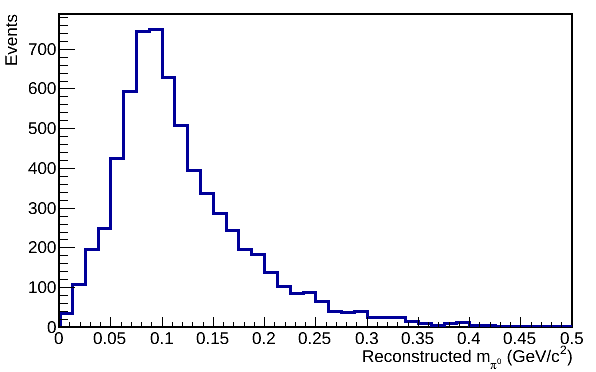
\includegraphics[width=0.8\textwidth]{pizeromass}
\end{cdrfigure}
\fixme{add figure; establish reference to calibration 
section; figure could also be at home in calibration section instead.}


\paragraph{PANDORA}
The reconstruction framework PANDORA~\cite{pandora} also works by
building up a three-dimensional picture from two-dimensional
reconstructed objects.  PANDORA is a flexible framework developed for
ILC detector simulation, and provides a convenient way to develop
algorithms for reconstructing particles.  In all, more than 80
algorithms, each targeting a specific topology, have been incorporated
into PANDORA to date.  Multiple passes through reconstructing the data
are possible.  Different criteria for clustering hits into tracks and
showers may be applied when seeking cosmic rays for removal rather than for
identifying signal events.  PANDORA proceeds by clustering hits in 2D,
reconstructing vertices in 3D, reconstructing tracks in 3D,
reconstructing showers in 3D, a mop-up step in 2D and 3D, followed by
full event building in 3D.

Plots of the efficiency and completeness for muons in charged-current $\nu_{\mu}$
events in MicroBooNE using PANDORA are shown in Figure~\ref{fig:muonpandoraperf}.
The resolution of vertex-finding is shown in
Figure~\ref{fig:pandoraresolution}.
%\fixme{Don't we have such a figure specifically for  protoDUNE ? If not, it should be a high priority task.}
% Answer: there won't be ccnumu events in protoDUNE.  Instead, vertices will arise from interactions of beam particles
% with the argon, and also cosmics.

\begin{cdrfigure}[Performance of PANDORA for muons in CC
  $\nu_mu$ events in MicroBooNE. ]{muonpandoraperf}{The performance of PANDORA for muons in charged-current
  $\nu_mu$ events in MicroBooNE. }
%\includegraphics[width=0.95\textwidth]{muonpandoraperf.png}\end{cdrfigure}
\end{cdrfigure}

\fixme{Include figure of PANDORA performance for muons.  Efficiency and
completeness (purity too if we can get the plot).}

\paragraph{PMA}
Another approach to 3D reconstruction in LArTPC detectors is referred to as the Projection Matching Algorithm
(PMA) ~\cite{pma_algorithm}. PMA was primarily developed as a technique for 3D reconstruction
of individual particle trajectories (trajectory fits) ~\cite{icarus3dreco}. Instead of
building up a 3D hypothesis from 2D clusters, it starts with the 3D hypothesis and compares
the 2D projection of the predicted trajectory of a particle with the observed data. Association
of hits between the 2D planes is not needed in this approach, improving its performance in
problematic cases, such as isochronous and short tracks.

PMA can take as input the output from different pattern recognition algorithms, from
LineCluster ~\cite{linecluster} to WireCell (described below).  Because these 2D algorithms
are run on each 2D projection independently, and because of detector defects,
clusters from  particles may be broken
into several smaller pieces, fractions of 2D clusters may be missing,
and clusters obtained from complementary projections are not guaranteed to cover corresponding
sections of trajectories. Such behavior is expected since ambiguous 
trajectories can be resolved only if the information from multiple 2D projections is used.
PMA performs higher level pattern recognition using as input clustering information from all
projections in order to search for the best matching combinations of clusters. The algorithm
also attempts to correct hit-to-cluster assignments using properties of 3D reconstructed objects.

PMA has been used successfully to reconstruct simulated beam particles in
\pdsp. In order to illustrate the performance of the entire reconstruction chain,
the spatial resolution of the interaction vertex with neutral pion
production, appearing in the 2~GeV/$c$ $\pi^+$ sample, is shown in Figure ~\ref{fig:PMApioninteraction}.
The resolution is found to be 0.6~\cm in this study.
A similar resolution is obtained also for the reconstruction
of inelastic interaction vertices in the 2~GeV/$c$ proton sample. 
%A study of the reconstruction performance
%for particles oriented in the same direction as beam particles was carried out as a check.

\fixme{A sentence on some known problems with specific directions would be useful to provide more background info for non-expert readers.}
Figures~\ref{fig:PMAproton2gevc}
and~\ref{fig:PMAcosmics} show examples of reconstruction of a 2~GeV/$c$ proton in the test beam and
cosmic-ray muons, respectively.

\begin{cdrfigure}[Vertex resolution for the
  inelastic interaction of $\pi^\pm$ mesons on Ar nuclei where a $\pi^0$ is produced]{PMApioninteraction}{Vertex position resolution in cm in $x$, $y$, and $z$ and 3D for the
  inelastic interaction of charged pions on liquid argon nuclei in events in which a $\pi^0$ is produced, in
  \pdsp, using the PMA algorithm.\fixme{increase size of stat box entries; if possible remove "temp" header}}
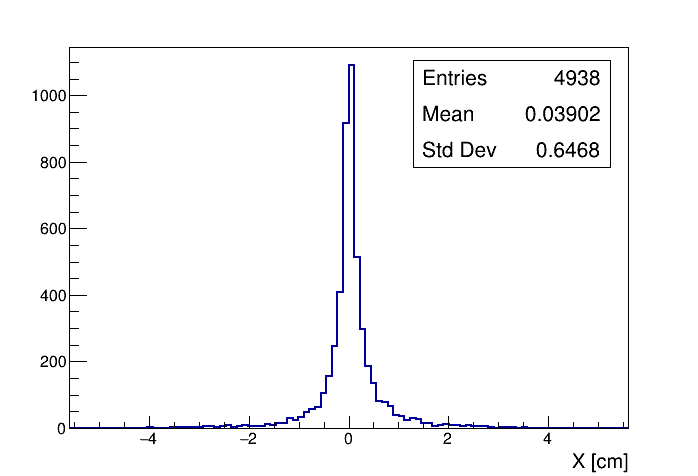
\includegraphics[width=0.45\textwidth]{pi0_vtx_dx.png}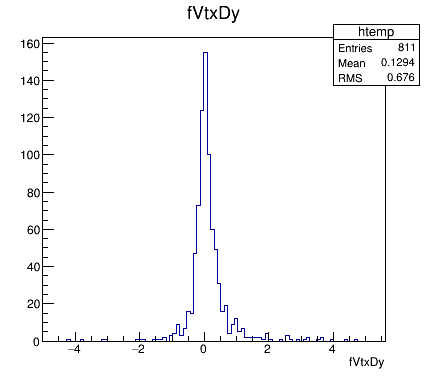
\includegraphics[width=0.45\textwidth]{figures/pi0_vtx_dy.png}
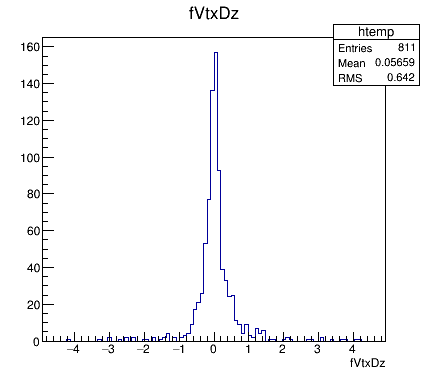
\includegraphics[width=0.45\textwidth]{pi0_vtx_dz.png}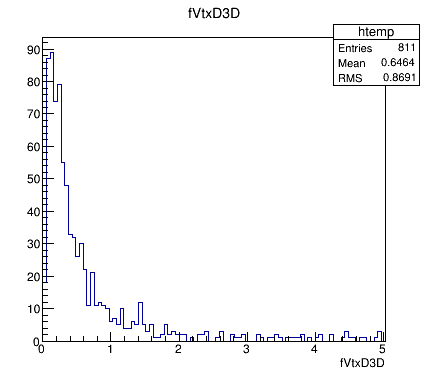
\includegraphics[width=0.45\textwidth]{figures/pi0_vtx3d.png}
\end{cdrfigure}


\begin{cdrfigure}[Example of reconstructed event of simulated proton with initial momentum 2 GeV/c]{PMAproton2gevc}{Example of reconstructed event of simulated proton with initial momentum 2 GeV/c (reconstruction algorithms: gaushit, Line Cluster and PMA).}
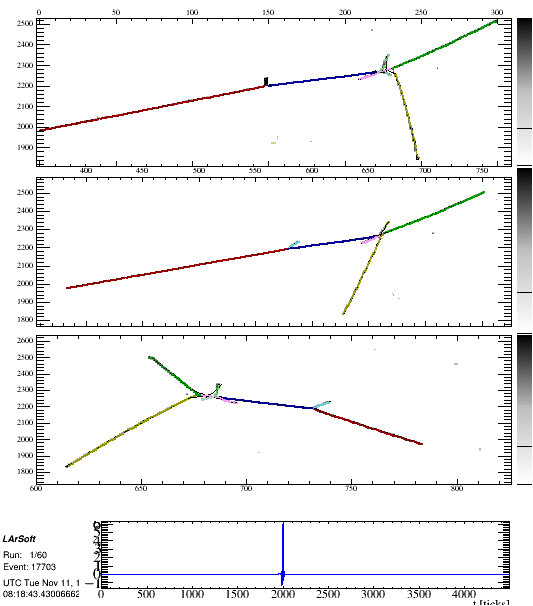
\includegraphics[width=0.45\textwidth]{figures/evdtwqproj117703.png}
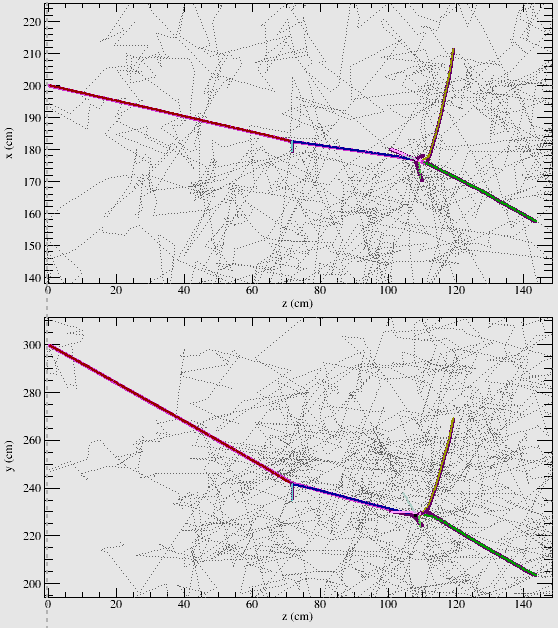
\includegraphics[width=0.45\textwidth]{figures/evdlarortho3d117703.png}
\end{cdrfigure}
\begin{cdrfigure}[Example of reconstructed cosmic muons in \pdsp]{PMAcosmics}{Example of reconstructed cosmic muons using gaushit, Line Cluster and PMA.}
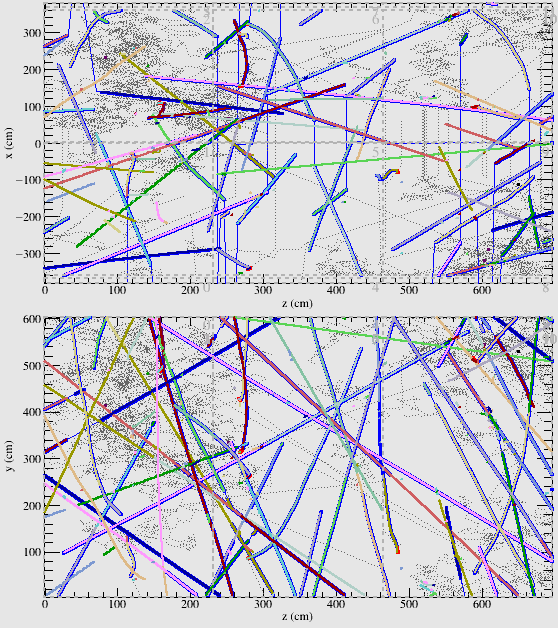
\includegraphics[width=0.45\textwidth]{figures/evdlarortho3d11302.png}
\end{cdrfigure}


%% Wire-Cell ... 
\paragraph{WireCell}
WireCell~\cite{wire-cell} adopts a very different approach from the 
aforementioned algorithms and is a new reconstruction method under development.
Instead of directly doing pattern recognition on each of the 2D views (drift 
time vs. wire number), the first step of the WireCell reconstruction is to 
perform 3D imaging with time, geometry, and charge information. The definition
of \textit{Hit} is based on signal strength after charge extraction (described in 
Sec.~\ref{sec:tpc-signal-calibration}) in a 2 $\mu$s time slice. 
The algorithm takes advantage of timing, geometry, and charge information in order to
suppress the effects of electronic noise.
Hits from  different wire planes arriving in different time 
slices cannot be associated with each other. Hits
from wires that do not cross in a region consistent with the charge deposition cannot be associated with each other. 
Hits from different wire planes
with different signal strengths are unlikely to be associated with each other. The 
usage of the charge information takes advantage of the fact that in a LArTPC with induction planes,
each of the wire planes in principle detects the same ionization electrons as the other planes. 
Figure~\ref{fig:quality} shows an example of the improvement of WireCell 3D imaging
over the more traditional approach. 

%
However, the suppression of the electronic noise comes at the cost of more
sensitivity to hit inefficiencies from dead channels or the signal processing steps.
 Since the track and shower hypotheses
are not used, the 3D imaging works for any event topology. 
Pattern recognition is needed to identify 
the content of these 3D images. Figure~\ref{fig:tracking2} shows the 
performance of the currently available 3D pattern recognition in
WireCell. For the long track going close to parallel to the wire plane, the reconstructed
track shows a zig-zag behavior. This is due to the current lack of a fine track fitting algorithm
that is expected to be added in the near future. 
Further developments of the WireCell pattern recognition algorithms
are needed before meaningful physics quantities can be calculated.
%
%% Wire-Cell Imaging
\begin{cdrfigure}[Comparison of imaging recon
qualities with and without charge information]{quality}{Comparison of imaging reconstruction 
qualities with and without the charge information. }
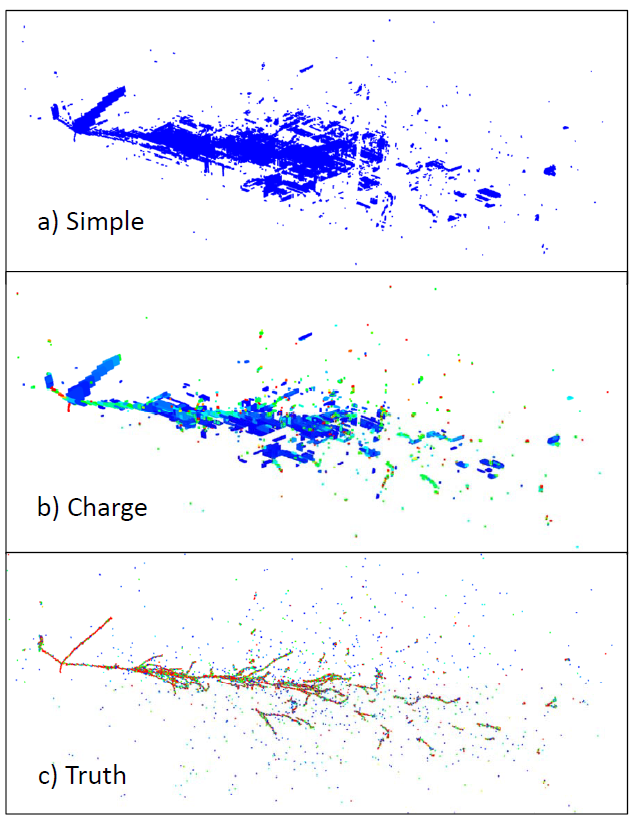
\includegraphics[width=0.5\textwidth]{quality.png}
\end{cdrfigure}
%
%
%% Wire-Cell 3D pattern recognition
\begin{cdrfigure}[Reconstructed image for one neutrino interaction event; comparison to MC]{tracking2}{The reconstructed image is shown 
on the left panel for one neutrino interaction event. The image 
was passed through the 3D pattern recognition program with tracks 
identified (middle panel). The identified pattern is compared 
with Monte-Carlo truth in the right panel. The zig-zag line in the right 
panel is the identified track.  More sophisticated track-fitting algorithms, to be added in the future,
will improve the track reconstruction.}
 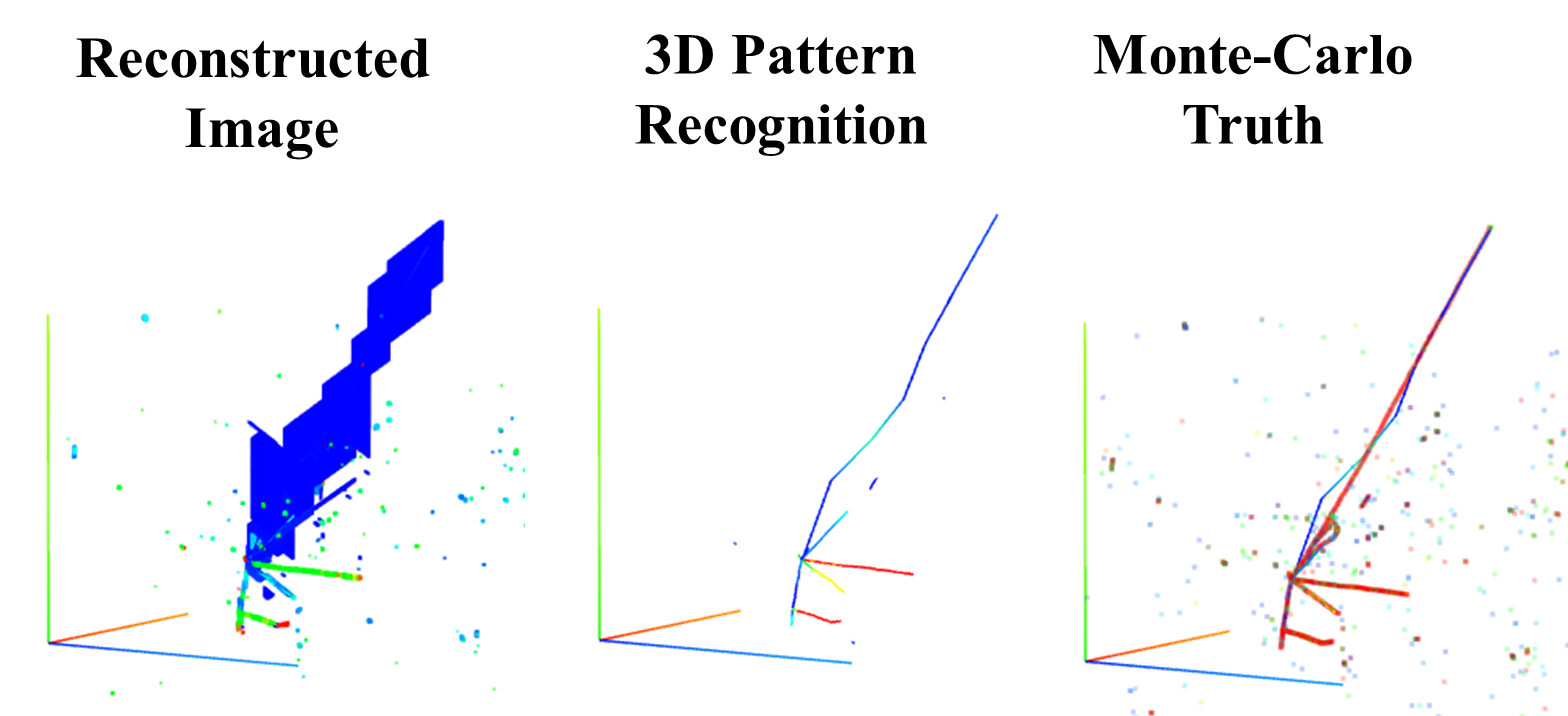
\includegraphics[width=0.9\textwidth]{Tracking_2.png}
\end{cdrfigure}

The \pdsp run will provide a large amount of raw data from a detector constructed with full-size DUNE
far detector components, installed in a test beam.  These data will provide a tremendous opportunity
to test the detector design, to test and optimize data processing and reconstruction techniques, and
to measure the properties of particle interactions in a liquid argon detector.  While the reconstruction
algorithms are currently still under development, the richness of the information provided by the detector
promises new opportunities to study the physics processes of charged particle and neutrino scatters.
